% Establece la clase del documento y las especificaciones de la misma.
\documentclass[28pt, a4paper]{report}

%%%%%%%%%%%%%%%%%%%%%%%%%%%%%%%%%%%%%%%%%%%%%%%%%%%%%%%%%%%%%%%%%%%%%%%%%%%%%%%%%%%%%%%%%%%%%%%%%%%%%%%%%%%%%%%%%%%%%%%%%%%%%%%%%

% Establece el tamaño de los bordes de la página.
\usepackage[top=2cm, bottom=2cm, left=1cm, right=1cm]{geometry}
% Permite el uso de hipervínculos en el documento.
\usepackage{hyperref}
% Establece que el documento va a ser escrito en español (méxico).
\usepackage[spanish]{babel}
% Permite el control sobre la Tabla de Contenidos, Figuras, etc.
\usepackage{tocloft}
% Fuente y Tipografía.
\usepackage[sfdefault,lf]{carlito}
% Asegura el uso de "Unicode Transformation Format 8-bit" para asegurar el uso de carácteres modernos.
\usepackage[utf8]{inputenc}
% Permite el uso de espaciado entre carácteres, líneas, etc.
\usepackage{setspace}
% Permite el uso de ítems con diferente forma.
\usepackage{enumitem}
% Permite el uso de textos alineados al centro, izquierda o derecha de la página.
\usepackage{ragged2e}
% Permite el uso de títulos, encabezados y pies de página.
\usepackage{titlesec}
% Permite el uso de un formato encabezados y pies de página de una forma más amigable al lector.
\usepackage{fancyhdr}
% Permite el uso de más colores.
\usepackage{xcolor}
% Permite el uso de Apéndices.
\usepackage{appendix}

%%%%%%%%%%%%%%%%%%%%%%%%%%%%%%%%%%%%%%%%%%%%%%%%%%%%%%%%%%%%%%%%%%%%%%%%%%%%%%%%%%%%%%%%%%%%%%%%%%%%%%%%%%%%%%%%%%%%%%%%%%%%%%%%%

% Permite la inserción de imágenes al archivo.
\usepackage{graphicx}
% Permite el uso de imágenes y figuras rotadas
\usepackage{rotating}
% Permite cambiar el tamaño de las imágenes.
\usepackage[export]{adjustbox}
% Permite el uso de hojas apaisadas y verticales.
\usepackage{pdflscape}
% Permite el uso de múltiples imágenes dentro de una figura.
\usepackage{subcaption}
% Permite la definición de objetos flotantes como tablas e imágenes.
\usepackage{float}
% Expande las capacidades de las tablas.
\usepackage{array}
% Expande las capacidades de las tablas.
\usepackage{tabularx}
% Expande las capacidades de las tablas.
\usepackage{tabularray}

%%%%%%%%%%%%%%%%%%%%%%%%%%%%%%%%%%%%%%%%%%%%%%%%%%%%%%%%%%%%%%%%%%%%%%%%%%%%%%%%%%%%%%%%%%%%%%%%%%%%%%%%%%%%%%%%%%%%%%%%%%%%%%%%%

% Permite el uso de ecuaciones y distintos formatos de las mismas.
\usepackage{amsmath}
% Permite el uso de fracciones de una forma que ocupe menos espacio y sea más legible.
\usepackage{graphicx, nicefrac}
% Permite el uso de cancelaciones en una ecuación.
\usepackage{cancel}
% Permite poner código como si fuera una términal de código.
\usepackage{listings}

%%%%%%%%%%%%%%%%%%%%%%%%%%%%%%%%%%%%%%%%%%%%%%%%%%%%%%%%%%%%%%%%%%%%%%%%%%%%%%%%%%%%%%%%%%%%%%%%%%%%%%%%%%%%%%%%%%%%%%%%%%%%%%%%%

% Establece que la carpeta a usar para almacenar las imágenes es "Imagenes".
\graphicspath{Imagenes/}

%%%%%%%%%%%%%%%%%%%%%%%%%%%%%%%%%%%%%%%%%%%%%%%%%%%%%%%%%%%%%%%%%%%%%%%%%%%%%%%%%%%%%%%%%%%%%%%%%%%%%%%%%%%%%%%%%%%%%%%%%%%%%%%%%

% Establece la separación entre líneas.
\setlength{\lineskip}{3.5pt}
% Establece la mínima separación entre líneas.
\setlength{\lineskiplimit}{2pt}
% Establece la sangría.
\setlength{\parindent}{20pt}
% Establece la separación entre parráfos.
\setlength{\baselineskip}{12pt}

%%%%%%%%%%%%%%%%%%%%%%%%%%%%%%%%%%%%%%%%%%%%%%%%%%%%%%%%%%%%%%%%%%%%%%%%%%%%%%%%%%%%%%%%%%%%%%%%%%%%%%%%%%%%%%%%%%%%%%%%%%%%%%%%%

\titleclass{\subsubsubsection}{straight}[\subsection]

\newcounter{subsubsubsection}[subsubsection]
\renewcommand\thesubsubsubsection{\thesubsubsection.\arabic{subsubsubsection}}
\renewcommand\theparagraph{\thesubsubsubsection.\arabic{paragraph}}

\titleformat{\subsubsubsection}
  {\normalfont\normalsize\bfseries}{\thesubsubsubsection}{1em}{}
\titlespacing*{\subsubsubsection}
{0pt}{3.25ex plus 1ex minus .2ex}{1.5ex plus .2ex}

\makeatletter
\renewcommand\paragraph{\@startsection{paragraph}{5}{\z@}%
  {3.25ex \@plus1ex \@minus.2ex}%
  {-1em}%
  {\normalfont\normalsize\bfseries}}
\renewcommand\subparagraph{\@startsection{subparagraph}{6}{\parindent}%
  {3.25ex \@plus1ex \@minus .2ex}%
  {-1em}%
  {\normalfont\normalsize\bfseries}}
\def\toclevel@subsubsubsection{4}
\def\toclevel@paragraph{5}
\def\toclevel@paragraph{6}
\def\l@subsubsubsection{\@dottedtocline{4}{7em}{4em}}
\def\l@paragraph{\@dottedtocline{5}{10em}{5em}}
\def\l@subparagraph{\@dottedtocline{6}{14em}{6em}}
\makeatother

\setcounter{secnumdepth}{4}
\setcounter{tocdepth}{4}

%%%%%%%%%%%%%%%%%%%%%%%%%%%%%%%%%%%%%%%%%%%%%%%%%%%%%%%%%%%%%%%%%%%%%%%%%%%%%%%%%%%%%%%%%%%%%%%%%%%%%%%%%%%%%%%%%%%%%%%%%%%%%%%%%

% Establece las condiciones para los hipervínculos.
\hypersetup{colorlinks=true,linkcolor=medium_violet,filecolor=dark_violet,urlcolor=light_violet,pdftitle={Carpeta Técnica GraviCap},pdfpagemode=FullScreen,}

%%%%%%%%%%%%%%%%%%%%%%%%%%%%%%%%%%%%%%%%%%%%%%%%%%%%%%%%%%%%%%%%%%%%%%%%%%%%%%%%%%%%%%%%%%%%%%%%%%%%%%%%%%%%%%%%%%%%%%%%%%%%%%%%%

% Establece el estilo de la página para permitir el uso de encabezados y pies de página.
\pagestyle{fancy}
% Establece el uso de encabezados y pies de página.
\fancyhf{}
% Establece el contenido de la parte izquierda del encabezado.
\lhead{\footnotesize \textcolor{dark_violet}{\textbf{GraviCap}} - \the\year{}}
% Establece el contenido de la parte central del encabezado.
\chead{
\includegraphics[width=1cm]{Imagenes/Preface/IMPA.png}}
% Establece el contenido de la parte de derecha del encabezado.
\rhead{\footnotesize E.E.S.T N°7 IMPA "T.R.Q."}
% Establece el contenido de la parte central del pie de página.
\cfoot{\large \thepage}

%%%%%%%%%%%%%%%%%%%%%%%%%%%%%%%%%%%%%%%%%%%%%%%%%%%%%%%%%%%%%%%%%%%%%%%%%%%%%%%%%%%%%%%%%%%%%%%%%%%%%%%%%%%%%%%%%%%%%%%%%%%%%%%%%%

% Establece que dentro de la tipografía "Carlito" se use la variante "OsF".
\renewcommand*\oldstylenums[1]{\carlitoOsF #1}
% Establece el tamaño del pie de página.
\renewcommand{\footrulewidth}{0.4pt}
% Establece que en la tabla de contenidos se use una línea de puntos para marcar el número de página.
\renewcommand{\cftsecleader}{\cftdotfill{\cftdotsep}}
% Establece un color con los valores 102, 19, 154 en RGB.
\providecolor{medium_violet}{RGB}{102,19,154}
% Establece un color con los valores 169, 68, 238 en RGB.
\providecolor{light_violet}{RGB}{169,68,238}
% Establece un color con los valores 81, 9, 129 en RGB.
\providecolor{dark_violet}{RGB}{81,9,129}

\definecolor{codegreen}{rgb}{0,0.6,0}
\definecolor{codegray}{rgb}{0.5,0.5,0.5}
\definecolor{codepurple}{rgb}{0.58,0,0.82}
\definecolor{backcolour}{rgb}{0.95,0.95,0.92}

%%%%%%%%%%%%%%%%%%%%%%%%%%%%%%%%%%%%%%%%%%%%%%%%%%%%%%%%%%%%%%%%%%%%%%%%%%%%%%%%%%%%%%%%%%%%%%%%%%%%%%%%%%%%%%%%%%%%%%%%%%%%%%%%%

\lstdefinestyle{mystyle}{
    backgroundcolor=\color{backcolour},   
    commentstyle=\color{codegreen},
    keywordstyle=\color{magenta},
    numberstyle=\tiny\color{codegray},
    stringstyle=\color{codepurple},
    basicstyle=\ttfamily\footnotesize,
    breakatwhitespace=false,         
    breaklines=true,                 
    captionpos=b,                    
    keepspaces=true,                 
    numbers=left,                    
    numbersep=5pt,                  
    showspaces=false,                
    showstringspaces=false,
    showtabs=false,                  
    tabsize=2
}

\lstset{style=mystyle}

%%%%%%%%%%%%%%%%%%%%%%%%%%%%%%%%%%%%%%%%%%%%%%%%%%%%%%%%%%%%%%%%%%%%%%%%%%%%%%%%%%%%%%%%%%%%%%%%%%%%%%%%%%%%%%%%%%%%%%%%%%%%%%%%%

\begin{document}
\begin{titlepage}

        \begin{center}      
            \begin{figure} [!ht]
                \centering
                
\includegraphics [width=9cm]{Imagenes/Preface/Logo-Nombre.png}
                \label{Logo-Nombre}
            \end{figure}
            {\Huge\textbf{Apéndices}}\par
                \vspace{0.2cm}
            {\LARGE\textbf{{\textcolor{dark_violet}{\textbf{GraviCap}}}}}\par
                \vspace{1.5cm}
            {\LARGE\textbf{7mo 1ra Comisión A}}\par
                \vspace{0.2cm}
            {\LARGE\textbf{Año \the\year}}\par
                \vspace{1cm}
            {\Large\textbf{{Alvarez Mollo, Fausto}}}\par
            {\Large\textbf{{Bianqui Kronemberger, Mariano Joaquín}}}\par
            {\Large\textbf{{Calleja, Tomás Joaquín}}}\par
            {\Large\textbf{{Donatti, Augusto}}}\par
            {\Large\textbf{{Felizia, Tatiana Milena}}}\par
            {\Large\textbf{{Sofía, Gabriel Jerónimo Takashi}}}\par
                \vspace{2cm}
            \begin{figure} [!ht]
                \centering
                
\includegraphics [width=7cm]{Imagenes/Preface/IMPA.png}
                \label{IMPA}
            \end{figure}
        \end{center}
        
    \end{titlepage}
    
%%%%%%%%%%%%%%%%%%%%%%%%%%%%%%%%%%%%%%%%%%%%%%%%%%%%%%%%%%%%%%%%%%%%%%%%%%%%%%%%%%%%%%%%%%%%%%%%%%%%%%%%%%%%%%%%%%%%%%%%%%%%%%%%%%%%%%%%%%%%%%%
    \tableofcontents
    \newpage
%%%%%%%%%%%%%%%%%%%%%%%%%%%%%%%%%%%%%%%%%%%%%%%%%%%%%%%%%%%%%%%%%%%%%%%%%%%%%%%%%%%%%%%%%%%%%%%%%%%%%%%%%%%%%%%%%%%%%%%%%%%%%%%%%%%%%%%%%%%%%%%

    \chapter{Apéndice A: Esquemáticos}
\renewcommand{\thepage}{A-\arabic{page}}
\setcounter{page}{1}
    Este apéndice presenta los esquemáticos eléctricos desarrollados para el proyecto \textcolor{dark_violet}{\textbf{GraviCap}}. Los esquemáticos incluidos proporcionan una visión detallada de los circuitos clave que permiten el funcionamiento eficiente del sistema. Estos esquemáticos son fundamentales para comprender la implementación de los sistemas de control y gestión de energía, y sirven como guía técnica para la construcción y funcionamiento del prototipo.
    Los dos esquemáticos que se incluyen en este apéndice son:\par
    
    \begin{itemize} [label = ]
    \setlength{\itemindent}{2em}
    
        \item MPPT (Maximum Power Point Tracking): Este esquema muestra el diseño del sistema encargado de optimizar la recolección de energía desde los paneles solares, asegurando que el sistema opere en el punto de máxima eficiencia, maximizando la energía capturada y transferida a la batería.\par
        \item Sistema de Control: Este esquema describe el hardware y la lógica de control del sistema de batería gravitatoria, incluyendo los componentes encargados de gestionar el flujo de energía entre la batería y la carga, así como los sensores que permiten un control preciso del sistema.\par
    \end{itemize}
    
    Ambos esquemáticos son esenciales para el correcto funcionamiento del sistema y proporcionan las bases técnicas para futuras expansiones o modificaciones en el diseño.\par

    \begin{landscape}
        \begin{sidewaysfigure}
            \centering
            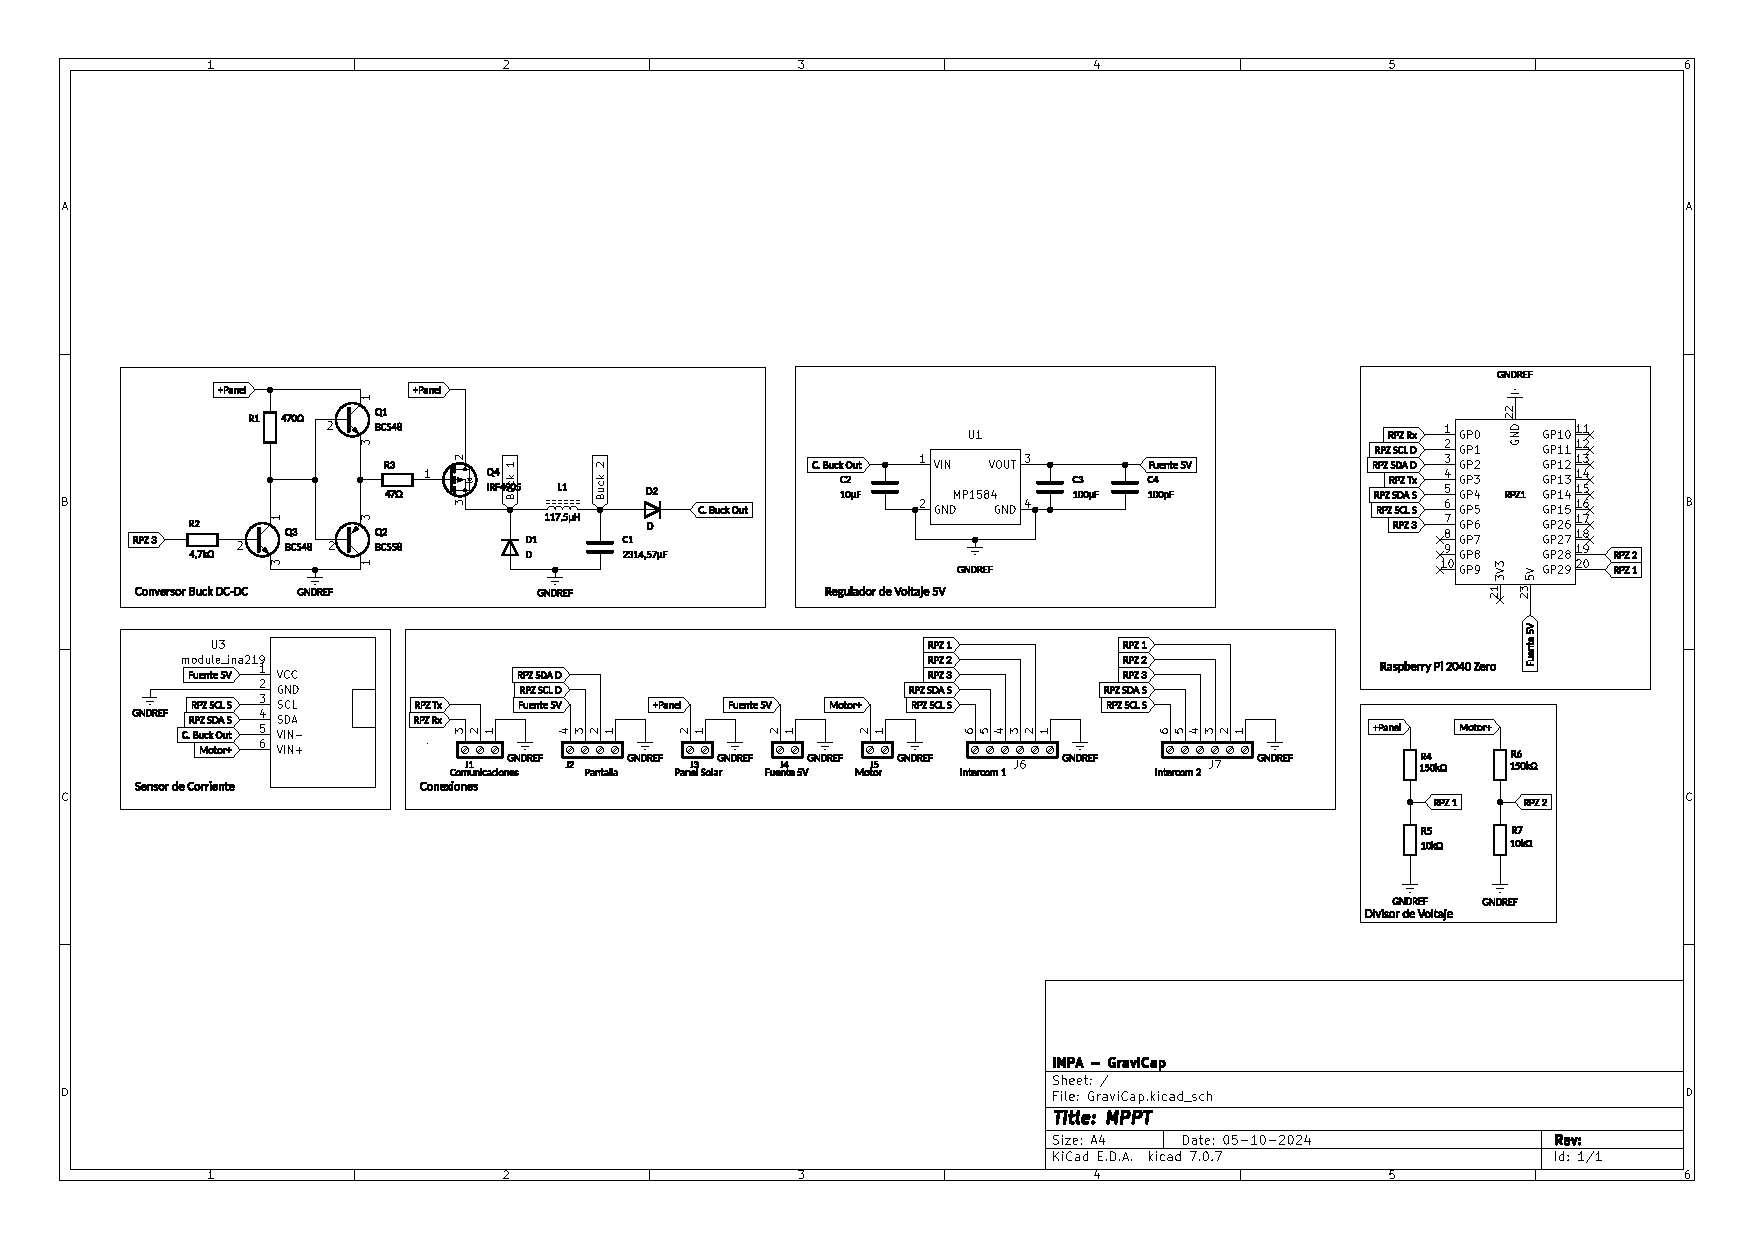
\includegraphics[angle=270, width=\textwidth,height=\textheight,keepaspectratio]{Anexo_A/Esquemático - MPPT.pdf}
            \label{fig:A_1}
        \end{sidewaysfigure}
        
        \newpage

        \begin{sidewaysfigure}
            \centering
            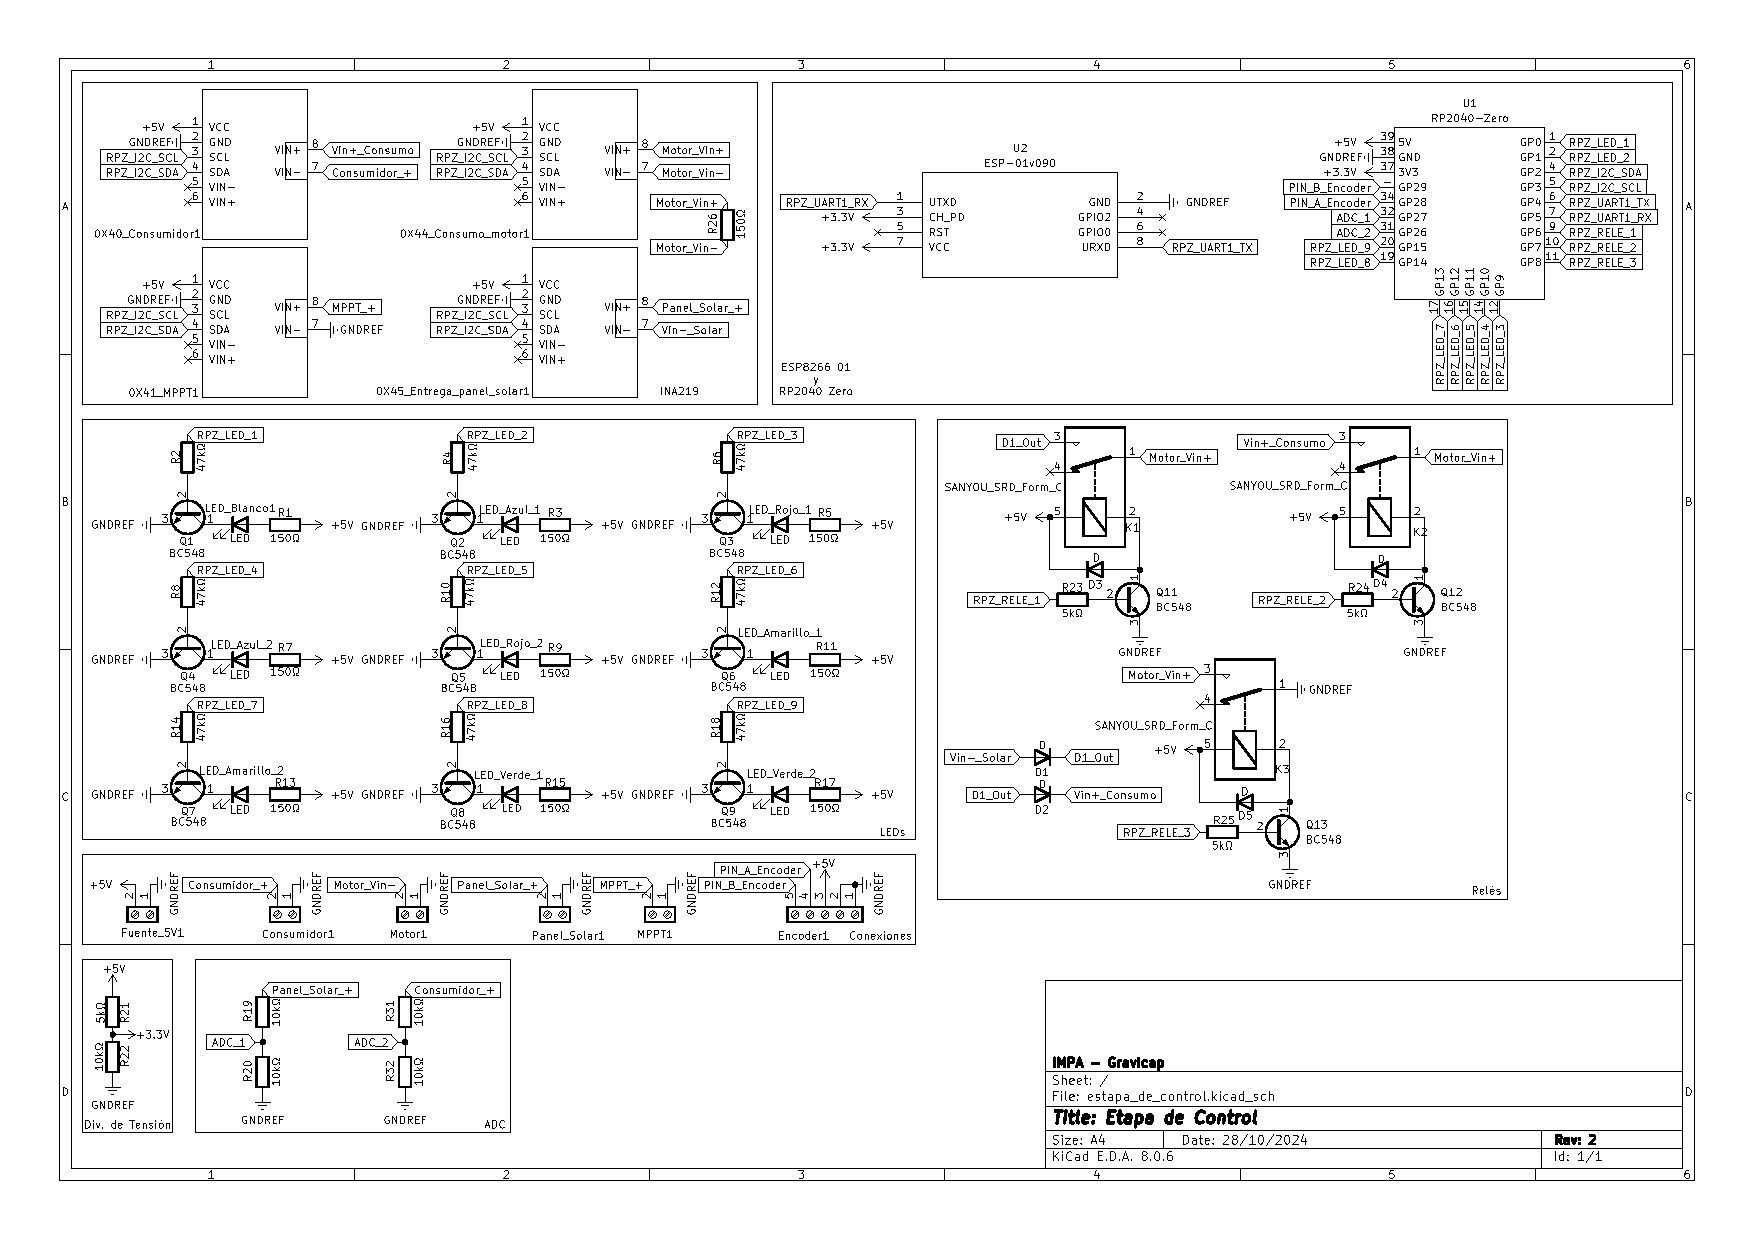
\includegraphics[angle=270, width=\textwidth,height=\textheight,keepaspectratio]{Anexo_A/Esquemático - Etapa_de_Control.pdf}
            \label{fig:A_2}
        \end{sidewaysfigure}
        
    \end{landscape}
    \chapter{Apéndice B: Códigos}
\renewcommand{\thepage}{B-\arabic{page}}
\setcounter{page}{1}
    \section{MPPT}
    
        \lstinputlisting[language=C, caption=\texttt{main.c} del MPPT]{main.c}
        \label{Listing B.1}
        
    \section{Etapa de Control}
        \lstinputlisting[language=C, caption=\texttt{main.c} de la Etapa de Control]{maino.c}
        \label{Listing B.2}
        
        \lstinputlisting[language=C, caption=\texttt{gravi.c} de la Etapa de Control]{gravi.c}
        \label{Listing B.3}

        \lstinputlisting[language=C, caption=\texttt{gravi.h} de la Etapa de Control]{gravi.h}
        \label{Listing B.4}
    \chapter{Apéndice C: Componentes}
\renewcommand{\thepage}{C-\arabic{page}}
\setcounter{page}{1}

    \section{RP2040 Zero}
    \label{rp2040}
            \begin{figure}[!ht]
                \centering
                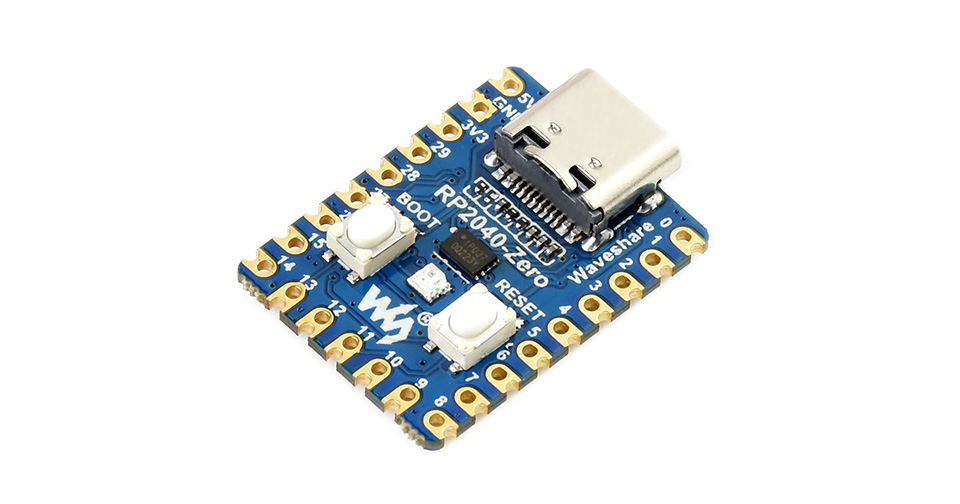
\includegraphics[width=0.7\linewidth]{Imagenes/Anexo_C/RP2040 Zero.png}
                \caption{RP2040 Zero}
                \label{fig:c1}
            \end{figure}
            
            Datos:\par
                \begin{itemize}[label=•]
                    \setlength{\itemindent}{2em}
                    
                    \item Chip microcontrolador RP2040 diseñado por Raspberry Pi en el Reino Unido\par
                    \item Procesador núcleo dual ARM Cortex M0+, con clock flexible que llega hasta los 133MHz\par
                    \item 264KB de SRAM, y 2MB de memoria Flash en la placa.
                    \item Conector USB-C, lo mantiene actualizado a los estándares actuales y más fácil de usar.\par
                    \item Los agujeros almenados permiten la soldadura directa a la placa.\par
                    \item USB 1.1 con soporte dispositivo/host.\par
                    \item Modos de suspención de bajo consumo y modo sleep.\par
                    \item Programación Drag-and-drop utilizando almacenaje en masa por USB.\par
                    \item 29 × pines GPIO multifunción (20× por vías externas, otros por puntos de soldadura).\par
                    \item 2 × SPI, 2 × I2C, 2 × UART, 4 × 12-bit ADC, 16 × canales de PWM controlables.\par
                    \item Clock y timer precisos en el chip.\par
                    \item Sensor de Temperatura.\par
                    \item Librerías     Accelerated floating-point en el chip.\par
                    \item 8 × Programmable I/O (PIO) state machines para soporte de periféricos personalizados.\par
                \end{itemize}
            
                Sitio Web: (\href{https://www.waveshare.com/wiki/RP2040-Zero}{https://www.waveshare.com/wiki/RP2040-Zero})\par
        
        \newpage
        
        \section{INA219}
        \label{ina219}
                \begin{figure}[!ht]
                    \centering
                    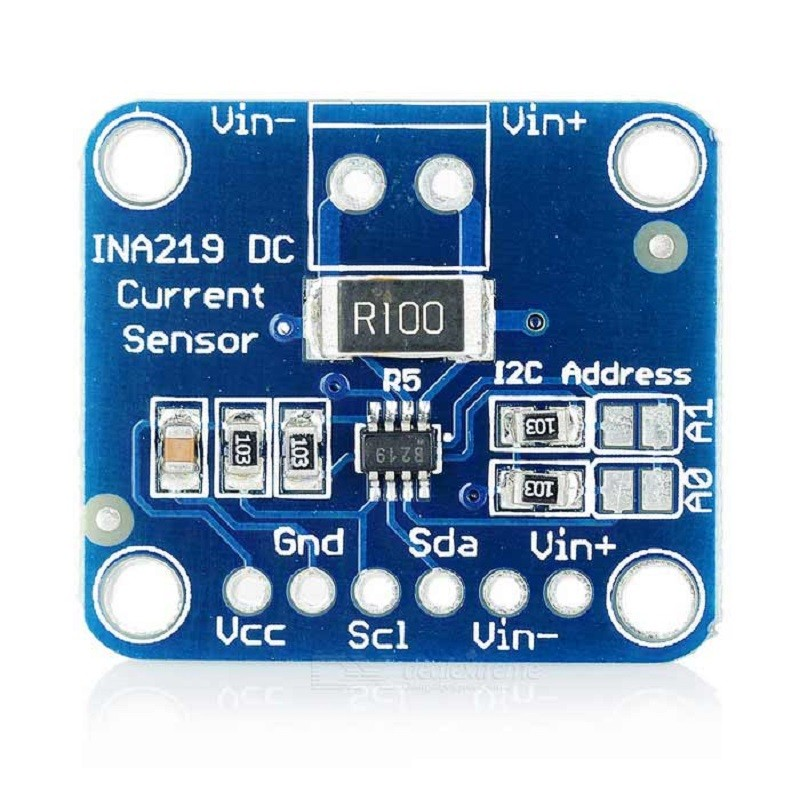
\includegraphics[width=0.7\linewidth]{Imagenes/Anexo_C/INA219.png}
                    \caption{Módulo INA219}
                    \label{fig:c2}
                \end{figure}
            
                Datos:\par
            
                \begin{itemize}[label=•]
                    \setlength{\itemindent}{2em}
                    
                    \item Entrada de potencia: 3,0V-5,5V\par
                    \item Voltaje objetivo hasta +26V\par
                    \item Resistencia de detección de corriente de 0,1 ohm 1\% 2W\par
                    \item Medición de corriente de hasta ±3,2A, con resolución de ±0,8mA\par
                    \item Detecta voltajes de bus de 0 a 26 V\par
                    \item Interfaz compatible con I2C- o SMBus-\par
                    \item Se pueden promediar hasta 128 muestras para lograr filtrado en entornos ruidosos.\par
                    \item Dimensiones de la Placa: 0.8 x 0.9 Pulgadas (l x w x h)\par
                \end{itemize}
            
                Datasheet: (\href{https://www.alldatasheet.com/datasheet-pdf/pdf/249609/TI/INA219.html}{https://www.alldatasheet.com/datasheet-pdf/pdf/249609/TI/INA219.html})\par

        \newpage
        
        \section{LPD3806-360BM}
        \label{encoder}
        
                \begin{figure}[!ht]
                \centering
                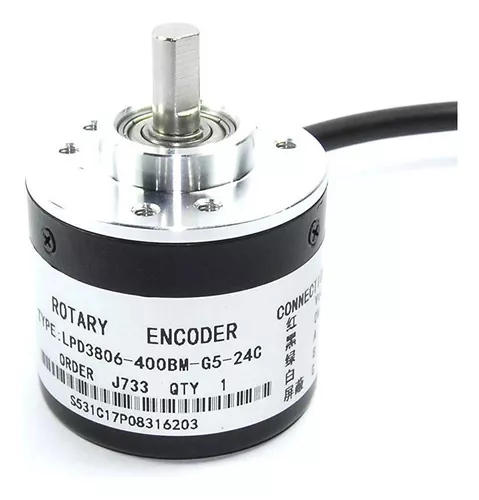
\includegraphics[width=0.5\linewidth]{Imagenes/Anexo_C/Encoder.png}
            \caption{LPD3806-360BM}
            \label{fig:c3}
        \end{figure}
        
            Datos:\par
            
            \begin{itemize}[label=•]
                \setlength{\itemindent}{2em}
                
                \item Pulsos: 600 p/r (600 pulsos/R monofasico, doble frecuencia de 4 a 2400 pulsos).\par
                \item Tension de Funcionamiento: 5V a 24V DC
                \item Eje: 6mm (Diametro) x 13mm (Largo)\par
                \item Dimensiones: 38mm x 35,5mm\par
                \item Salida de Pulso ortogonal rectangular con salida 2 fases AB\par
                \item Salida de colector abierto NPN\par
                \item Velocidad Mecanica Maxima: 5000rpm.\par
                \item Frecuencia de respuesta: 0-20kHz\par
            \end{itemize}
            
            Datasheet: (\href{https://www.alldatasheet.com/datasheet-pdf/pdf/1150705/ETC2/LPD3806-360BM.html}{https://www.alldatasheet.com/datasheet-pdf/pdf/1150705/ETC2/LPD3806-360BM.html}) (Está en Chino)\par

    \newpage
    
    \section{ESP8266 ESP-01S}
    \label{esp8266}
        \begin{figure}[!ht]
            \centering
            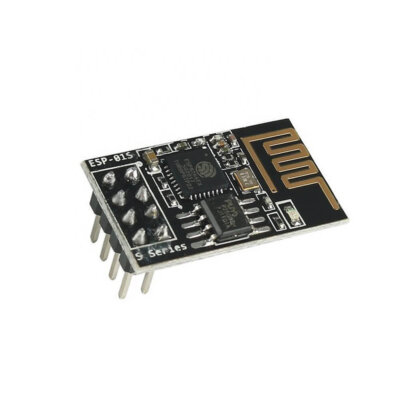
\includegraphics[width=0.5\linewidth]{Imagenes/Anexo_C/ESP8266.png}
            \caption{Módulo ESP8266 ESP-01S}
            \label{fig:c4}
        \end{figure}
        
        Datos:\par
        
        \begin{itemize}[label=•]
            \setlength{\itemindent}{2em}
            
            \item Voltaje de alimentación: 3.3 V. Este módulo no tolera 5 V.\par
            \item Comunicación tipo de interfaz: Serial, UART\par
            \item CPU de 32 bits\par
            \item Frecuencia de Reloj: 80MHz/160MHz\par
           \item Instruction RAM: 32KB\par
            \item Data RAM: 96KB\par
            \item Memoria Flash Externa: 4MB\par
            \item Soporte 3 modos: AP, STA, AP + STA\par
            \item Wi-Fi Direct (P2p), soft-AP\par
            \item Protocolos soportados: 802.11 b/g/n –  TCP/IP\par
            \item Soporte de red: 2,4 GHz\par
            \item Perfecto y simple en comandos AT\par
        \end{itemize}
            
        Datasheet: (\href{https://www.alldatasheet.com/datasheet-pdf/pdf/1424861/ETC/ESP8266.html}{https://www.alldatasheet.com/datasheet-pdf/pdf/1424861/ETC/ESP8266.html})\par
    
\end{document}